\documentclass{article}
\usepackage[utf8]{inputenc} 
\usepackage{graphicx} 
\usepackage{float} 
\usepackage{hyperref} 

\title{Thesis Log} 
\author{Nikunj Gupta}
\date{August 2018}

\begin{document}

\maketitle 
\section{Week 1 (August 22) } 
\begin{itemize}
	\item Recap 
	\item Look at literature survey 
	\item Data set 
\end{itemize}

\section{Week 2 (August 29)} 
\begin{figure}[h]
	%\hspace{-3.0cm}
	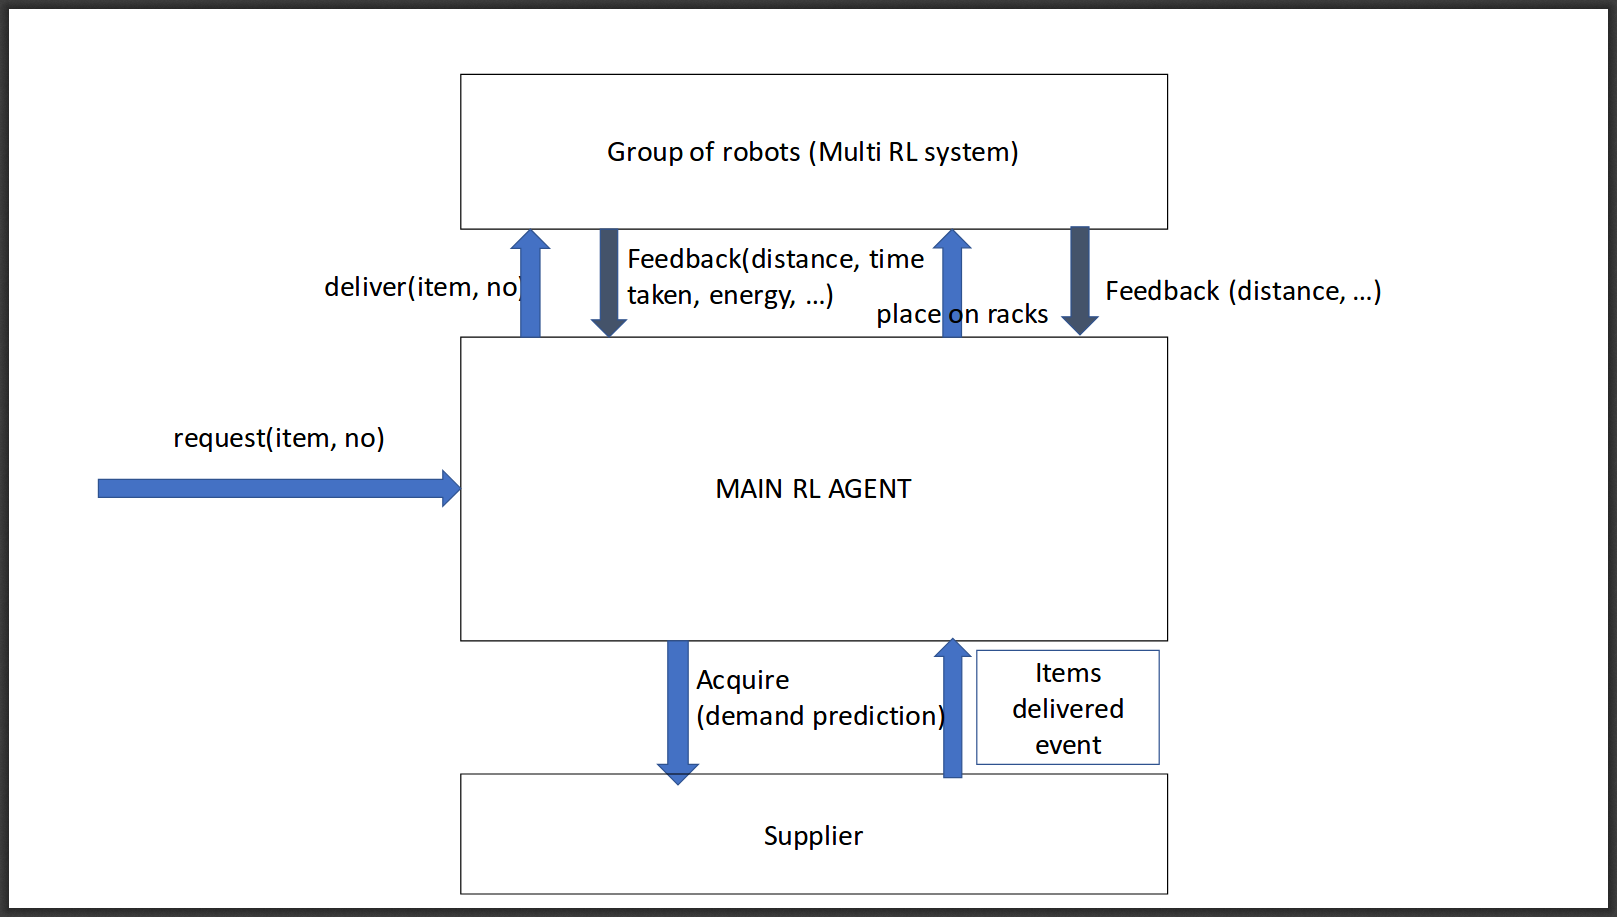
\includegraphics[width=13.5cm]{workflow/workflow.png} 
	\centering 
\end{figure} 
\textbf{Discussion: } To be updated...

\begin{itemize}
	\item A comprehensive survey of MARL: Reading 
	\item Data sets 
	\item Demand Forecasting Survey - papers and tools 

\end{itemize}

\section{Week 3 (September 5) } 
	Discussion: The paper: "A Comprehensive Survey of MARL Algorithms" mentions a lot of issues and research problems in multi-agents in reinforcement learning. Also, there are some more papers addressing the same and can be read for more understanding (mentioned below). \newline 
	In MARL, there are many cases like the agents are fully cooperative or fully competitive or of mixed nature. We will have to decide upon what form of MARL we will be requiring for our problem. Some aspects ensure distributed sort of solving any problem, whereas the others handle the environments as a single central system. Other practical issues which the paper mentions is regarding the scalability of the agents. Till then (2007), only a small scale problem was solvable using any of the algorithms mentioned in the paper. There has been some work done in this direction though. 
	
	\subsection{References} 
	\begin{itemize}
		\item  \href{https://docs.google.com/presentation/d/1OhF0KokVcQkeHrQPxT7xzA1GClhjhw3srpNi-78n5Oc/edit?usp=sharing}{Presentation on A Comprehensive Survey of Multi-Agent Reinforcement Learning} 
		\item \href{https://ieeexplore.ieee.org/document/4445757/}{A Comprehensive Survey of Multi-Agent Reinforcement Learning} 
		\item Further reading: Reference numbers from above paper: 123, 125, 128, 130. 
	\end{itemize} 
	




\end{document}